\documentclass[10pt,letterpaper]{article}
\usepackage[margin=0.68in,top=0.72in,bottom=0.72in]{geometry}
\usepackage[T1]{fontenc}
\usepackage[scaled=0.96]{helvet}
\renewcommand{\familydefault}{\sfdefault}
\usepackage{amsmath,amssymb,array,booktabs,tabularx,tikz,fancyhdr,enumitem}
\usepackage[hidelinks]{hyperref}
\urlstyle{same}
\usetikzlibrary{arrows.meta,calc}
\setlength{\parindent}{0pt}
\setlength{\parskip}{6pt}
\setlist[itemize]{leftmargin=15pt,itemsep=3pt,topsep=3pt}
\setlist[enumerate]{leftmargin=18pt,itemsep=3pt,topsep=3pt}
\pagestyle{fancy}\fancyhf{}
\fancyhead[L]{\small Week 64 / Straight paths on strange surfaces / Adult guide}
\fancyfoot[L]{\small Bellingham Math Circle / Week 64 / W64-FAC-v1}
\fancyfoot[R]{\small\thepage}
\renewcommand{\headrulewidth}{0.3pt}\renewcommand{\footrulewidth}{0pt}
\setlength{\headheight}{14pt}\setlength{\headsep}{15pt}\setlength{\footskip}{18pt}
\renewcommand{\arraystretch}{1.15}
\newcommand{\topic}[1]{\vspace{3pt}{\large\bfseries #1}\par}
\newcommand{\labelled}[2]{\textbf{#1} #2\par}
\newcommand{\hint}[1]{\textbf{Hints, in order.} #1\par}
\newcommand{\route}[1]{\textbf{Route.} #1\par}
\newcommand{\octagon}{\draw[line width=.7pt] (1,2.41421356)--(2.41421356,1)--(2.41421356,-1)--(1,-2.41421356)--(-1,-2.41421356)--(-2.41421356,-1)--(-2.41421356,1)--(-1,2.41421356)--cycle;}
\definecolor{pathblue}{RGB}{24,88,148}
\begin{document}
\topic{Mathematical destination: the facts behind the experiments}
\labelled{Translation preserves a heading.}{Glue each side of a regular octagon to the opposite side by a translation: corresponding points are the same point of the surface. A traveler exits at one point and resumes at its mate, keeping the same direction. There is \textbf{no reflection and no turn}. Position \emph{on the surface} and heading must both return for a closed trip. At a vertex, stop: the directional flow has no unique continuation there. [S1]}
\labelled{Horizontal trips form two families.}{Use an octagon with side length 2, centered at the origin, with horizontal and vertical sides. Put \(a=1+\sqrt2\), \(b=2+\sqrt2\). For \(-1<y<1\), rightward trips close after one edge crossing and have length \(2a\). For \(1<y<a\), a trip visits an upper and a lower strip, closes after two crossings, and has length \(2b\). The lower strip belongs to the same family. Each whole loop has the same length within its family, although its separate drawn segments vary. Lines through vertices are excluded. Children can compare with tracing strips, without square roots.}
\labelled{Eight corners become one exceptional point.}{Endpoint matching identifies all eight vertices. Each contributes \(135^\circ\); together they give \(1080^\circ\), or \emph{three full turns}. Away from this point the surface is Euclidean-flat, including across joined edges. Its one-face, four-edge, one-vertex description has Euler characteristic \(-2\), so the connected closed orientable surface has genus 2. The two-handle conclusion uses a classification theorem; it is adult context, not something proved by a sketch. [S1]}
\labelled{The three-square L has the same topology, a different geometry.}{Label its lower-left, lower-right and upper-left squares A, B and C. Right-edge crossing swaps A/B and fixes C; top-edge crossing swaps A/C and fixes B. The twelve square-corner sectors form one \(1080^\circ\) cone point. Again the genus is 2, but this is a different flat metric. The L is not a regular octagon cut into three equal squares. [S2, S3]}
\labelled{Rational directions close in the square model if they avoid corners.}{A rational direction repeats its local coordinates on the unit square after a fixed displacement block. That block permutes the finitely many square labels, so some repetition returns the entire state. Returning to the same local dot in a different square is insufficient. The proof is for the square-tiled model; it does \textbf{not} supply a rational/irrational slope test for the regular octagon. Finite drawings prove neither density nor ergodicity.}
\labelled{Two different octagon pictures must stay separate.}{Translated regular Euclidean octagons can overlap in a route drawing; they do not tile the ordinary plane. The usual hyperbolic genus-two octagon tiling uses a different metric, with \(45^\circ\) corners when eight meet smoothly. Our octagon has \(135^\circ\) corners and a cone point. [S4]}
\topic{What children are meant to discover}
Make and check a portal crossing; find and compare complete trips; notice that moving the start can change a trip or preserve its total length; chase corner identifications; then use an exact square lab to explain return through a finite set of states. A drawing is an \textbf{experiment}; a proposed rule is a \textbf{conjecture}; a matching argument or exact calculation is an \textbf{explanation}.
\par\begin{tabularx}{\linewidth}{@{}p{1.06in}X@{}}
\toprule
Entry & Readiness, independent of grade \\
\midrule
Grades 3--5 core & Match edge letters and arrows; move a ruler without turning; compare positions along equal edges; retain a start dot and travel arrow. Adult reading/recording is fine. No degree measure, fractions, algebra or square roots is required. \\
Later routes & Corner work needs endpoint matching and sector counting. The L lab needs square labels, grid positions and a repeated direction step. The general return proof needs reversible moves; adult formulas are not prerequisites. \\
\bottomrule
\end{tabularx}
\newpage
\topic{Prepare a small, usable kit}
\labelled{Per pair or trio.}{Student pages for the chosen route, 3--5 sheets of tracing paper or translucent baking paper, a ruler, pencil/eraser, two colored pencils, plain paper, one small movable counter, and a separate short paper direction arrow. Have scissors for the corner sectors; an adult can cut. A spare printed copy preserves an example while the next trial is made.}
\labelled{Printing and space.}{Print single-sided on US Letter: pp. 1--2 per pair for a first visit; p. 3 and tracing sheets for developing; pp. 4--5 for corners, keeping p. 4 uncut; pp. 6--9 only as chosen. Match traced copies to their original size; check the p. 5 scale before cutting. The optional three-copy p. 3 layout needs about 12 by 8 inches of desk. Never stretch the octagon's axes independently. No child needs to fold it into a two-handled object.}
\labelled{Staffing and roles.}{Use pairs wherever possible. The traveler chooses or draws the path; the checker points to the matching edge, locates the corresponding point, and checks the unchanged direction. Swap after a complete trial. In a trio, rotate a recorder who preserves one path and its start arrow. An adult may read, steady tracing paper, or record a dictated observation; children should still choose and check the path.}
\labelled{Before children arrive.}{Select a short route and read its answers. Trace one working octagon, including edge labels, matching arrows and a clear top mark. Keep a loose direction arrow next to it. Separate unused pages so that a thick packet does not become a completion demand. Preparation needs ordinary printing and tracing, not a custom three-dimensional model.}
\labelled{Physical rehearsal still needed.}{Try a slanted-edge transfer with the actual print, ruler and tracing paper. Check that labels remain visible through the paper; corresponding fractions of an edge are easy to match; children can keep the direction arrow fixed while moving a counter; corner marks and grid dots remain distinguishable. Test sector cutting and handling. \textbf{These materials are unpiloted. Digital checks do not establish physical fit or classroom usability.}}
\topic{A shared launch: slide the map, keep the heading}
\labelled{Handle first, about 2 minutes.}{Let children move a counter and trace a little of the octagon. Ask one child to find matching edges. Point out that the small printed edge arrows tell which points correspond; the loose arrow tells where the traveler is going. They do different jobs.}
\labelled{Show one legal crossing, about 3 minutes.}{Use the student packet's non-task visual. On a spare octagon, approach a nonvertex point on the right vertical edge along a short slanting line. Stop at the edge. Match its position on the left edge, measured from the same end of the identically directed arrows. Move the counter to its mate and draw the next short segment \emph{parallel to the first}, traveling in the same direction. Do not finish a loop or announce the length rule.}
\labelled{Show why the pieces are straight.}{Trace the octagon on transparent paper. Slide, do not turn or flip, the copy until its left edge lies on the original right edge. The arrival segment and continued segment now lie on one ruler line. Mark the copy 2. In the original drawing, the resumed piece belongs at the matched left-edge point. Physical overlap never tells us which surface points are equal; edge labels do.}
\labelled{Children demonstrate the rule.}{A volunteer makes one crossing at a different point. The checker touches both corresponding points, then compares travel arrows. Say: Same place on the matching arrow, same heading. If you reach a corner, stop. A trip is back only at its own starting point with its starting heading. Give pairs their first selected task.}
\labelled{Keep one visible record.}{A path with its starting dot, direction arrow and numbered crossings is enough. Do not demand a crossing tally, code, distance sum and oral explanation simultaneously. Save the paper so another pair can check it.}
\newpage

\topic{A short first route, with real return visits}
\labelled{First visit.}{Allow the usual arrival/movement time, then about 5 minutes for handling and the shared crossing. Give pairs student p. 1 for 10--15 minutes, then p. 2 for 15--20 minutes if the rule is secure. Close with 5 minutes comparing two saved trips. One carefully checked trip and a conjecture can be a good stopping point. If time and attention remain, start p. 3; completing every page is not the aim.}
\labelled{Return visit: one straight developed line.}{Reestablish one crossing, then give p. 3 a full 15--25 minutes. Compare complete two-piece loops, move the start, and check how separately numbered copies make the line straight. This adds a representation for explaining the portal rule.}
\labelled{Return visit: the exceptional point.}{Use pp. 4--5 together. Allow 10--15 minutes for endpoint matching and another 15--20 for cutting, ordering and counting sectors. Keep an uncut p. 4 beside the pieces; precut p. 5 if cutting would use the whole session. This is a different question from path tracing.}
\labelled{Return visit: exact returns.}{Start the L model on p. 6, with its new square labels and outside edge pairs. Continue to p. 7 or p. 8 when children can check that rule. Save p. 9 and the universal explanation for a later visit if needed. Each deserves 15--25 minutes, not a final five-minute challenge. The p. 9 proof is a readiness-dependent Grades 4--5 extension.}
\labelled{If the rule is too much.}{Return to one crossing at a time, with a partner controlling the direction arrow and an adult steadying a tracing. If the adult must choose every point and direction, stop the independent investigation and use a familiar activity. This packet makes no K--1 entry claim.}
\topic{Student p. 1 / Problem 1: three marked trips}
\route{Concrete entry. All three marked rightward paths close; none hits a corner. Edge letters A, B, C, D refer to printed pairs, not the later L-square names.}
\begin{tabularx}{\linewidth}{@{}p{.40in}p{1.3in}X@{}}
\toprule
Start & Crossings in order & Full answer \\
\midrule
P & C & Stays in the middle band; one loop is the full left-to-right width. \\
Q & B, D & Runs through the upper and lower bands; two crossings before returning to Q. \\
R & D, B & Runs through lower and upper bands; two crossings before returning to R. \\
\bottomrule
\end{tabularx}\par
\labelled{Exact check.}{In the background coordinates, \(P=(-.65,0)\), \(Q=(-.3,1.60)\), \(R=(.20,-1.45)\). P has length \(2a\). Q and R each have length \(2b\), although their paired chords differ. Q's lower height is \(1.60-b\); R's upper height is \(b-1.45\). These are distinct loops in the same outer family.}
\hint{1. Have the checker identify the mate before moving. 2. Trace the edge and mark its crossing point, then slide that tracing to the paired edge without rotation. 3. When the route crosses its starting horizontal line, keep going until it reaches the actual starting dot.}
\topic{Student p. 2 / Problem 2: classify all interior starts}
\labelled{Complete answer.}{There are exactly two closed-trip lengths. Starts strictly between the horizontal lines through the vertical-edge endpoints give the shorter \(2a\) loop. Starts strictly above or below that central band give the longer \(2b\) loop. Interior starts on the two dividing lines hit a corner and stop. No other interior cases exist; the horizontal coordinate only changes where the loop begins.}
\labelled{Measurement.}{On this p. 2 octagon, printed width is 5.35 inches. At actual size, short loops measure 5.35 inches and long loops \(5.35\sqrt2\approx7.57\) inches. These are full traveled lengths, with jumps excluded and the final piece included. Never compare inches across different-sized pages.}
\hint{1. Compare a near-top start with a central one. 2. Trace both pieces of a complete outer trip onto one strip. 3. Move a start vertically and look for where its exit edge changes. The formula \(2(b-y)+2y\) explains why measurements that look nearly equal really are equal.}
\newpage
\topic{Student p. 3 / Problem 3: a balanced loop, drawn straight}
\route{First substantial extension or return visit. The printed task starts on an edge, away from a corner, so one trip consists of two complete chords.}
\labelled{Answer.}{The upper and lower chords must have equal length. In side-length-2 coordinates, their heights are \(y=\pm b/2=\pm(2+\sqrt2)/2\); each chord has length \(b\). Start at the midpoint of the upper-left D edge, heading right. Exit at the upper-right B midpoint, resume at the lower-left B midpoint, and cross the lower chord to the lower-right D midpoint. This is the matching point of the starting edge, with the same heading: one full trip. A lower-left B midpoint start gives the same loop in the other order.}
\labelled{Printed seam-start development.}{Use copy 1 at its original position and copy 2 translated by \((b,b)\), putting its SW B edge on copy 1's NE B edge. The straight line from \((-b/2,b/2)\) to \((3b/2,b/2)\) traverses the two full chords. Its final point, on copy 2's D edge, matches the original start. A third copy may mark that correspondence, but its interior is not needed for the completed trip.}
\labelled{Optional interior-start variant, shown below.}{After the printed task, move the start to \(S=(0,b/2)\). Keep copy 2 as above and translate copy 3 by \((2b,0)\), matching its NW D edge to copy 2's SE D edge. The line at \(y=b/2\) reaches the same local point \(S\) in copy 3 after distance \(2b\). This variant has three drawn pieces because one complete chord is split at the start.}
\begin{center}
\begin{tikzpicture}[scale=.54,>=Stealth,every node/.style={font=\small}]
\begin{scope}\octagon\node at (0,-.35){copy 1};\end{scope}
\begin{scope}[shift={(3.41421356,3.41421356)}]\octagon\node at (0,.55){copy 2};\end{scope}
\begin{scope}[shift={(6.82842712,0)}]\octagon\node at (0,-.35){copy 3};\end{scope}
\draw[pathblue,line width=1.4pt,->] (0,1.70710678)--(6.82842712,1.70710678);
\foreach \x in {0,1.70710678,5.12132034,6.82842712}{\fill[pathblue] (\x,1.70710678) circle(2.2pt);}
\node[below] at (0,1.52){start \(S\)};
\node[below] at (1.70710678,1.70710678){B};
\node[below] at (5.12132034,1.70710678){D};
\node[below] at (6.82842712,1.52){return \(S\)};
\end{tikzpicture}
\end{center}
\labelled{Why three copies in the optional picture?}{An interior start cuts the upper chord into an initial and final piece. Here their lengths are \(b/2+b+b/2=2b\). A different interior start changes the first and last lengths, keeping their sum \(b\). The printed seam-start route instead uses two whole chords. In either drawing the final point represents the starting surface point, even though it lies elsewhere on the desk.}
\hint{1. Compare the complete upper and lower chords, not the first piece from the dot. 2. Move the upper height until neither piece looks longer. 3. Try the midpoint of a sloping edge and check its mate. For developing, align two labeled edges first; then move the ruler.}
\labelled{Checks to ask for.}{Copies must not rotate or flip; the developed path is one line. Start and return must be matching surface points with the same arrow. The printed convention uses two whole chords; an independently correct interior-start drawing is a useful variant, not a failure. Do not demand a plane-filling pattern. If later copies overlap, keep their sheet identities distinct.}
\labelled{An explanation without algebra.}{Mark the upper and lower pieces on tracing strips. Move the upper line upward a little: both sloping ends move inward, while the partnered lower line expands by the same amount. At the balanced middle position the two strips match. The midpoint construction gives an exact check of an experimental guess.}
\newpage
\topic{Student p. 4 / Problem 4: which corners are one point?}
\route{Corner-identification investigation. Keep each polygon flat and trace its endpoint matches. Keep the uncut diagrams visible for the next problem.}
\labelled{Octagon answer.}{One group contains all eight corners: \(\{1,2,3,4,5,6,7,8\}\). The complete endpoint pairs, using printed labels, are
\[
\begin{array}{c|cc}
\text{edge pair}&\multicolumn{2}{c}{\text{endpoint matches}}\\ \hline
A&8\sim5&1\sim4\\
B&1\sim6&2\sim5\\
C&3\sim6&2\sim7\\
D&4\sim7&3\sim8.
\end{array}
\]
For a single checkable tour through the group, use \(1\to6\to3\to8\to5\to2\to7\to4\to1\). Every arrow is an allowed endpoint match, not a drawn path through the polygon's interior.}
\labelled{Square answer.}{One group contains all four corners: \(\{9,10,11,12\}\). E matches \(12\sim11\), \(9\sim10\); F matches \(10\sim11\), \(9\sim12\). A tour is \(9\to10\to11\to12\to9\). The two separate shapes are separate surfaces; do not combine corners 1--8 with 9--12.}
\hint{1. Choose one edge letter and match arrow tails, then heads. 2. Start a corner card group with one forced pair. 3. When one number occurs in two groups, combine the groups. Keep going until all pairs have been checked.}
\labelled{Important distinction.}{The octagon and square both produce one corner group. That fact alone does not make their local geometry the same. Problem 5 asks how much corner angle belongs to that point.}
\topic{Student p. 5 / Problem 5: how many turns around the point?}
\labelled{Answer and order.}{Arrange octagon sectors in order \(1,6,3,8,5,2,7,4\), closing back to 1, or in reverse cyclic order. Any rotation of this list is equivalent. The sequence of seams is B, C, D, A, B, C, D, A. Square sectors can follow \(9,10,11,12\), closing to 9, with seams E, F, E, F. Rotate the pieces to join corresponding rays; keep both their labels and arrow directions matched.}
\labelled{Angle result.}{The eight \(135^\circ\) sectors give \(1080^\circ\), exactly \textbf{three full turns}. The four \(90^\circ\) sectors give \(360^\circ\), \textbf{one full turn}. Children need not name degrees: an octagon corner is three eighth-turn pieces, so all eight give 24 eighths, or three turns. Each square corner is a quarter-turn.}
\hint{1. First make the ordinary square corner neighborhood. 2. Use that full turn as a reference for the octagon pieces. 3. Count all numbered sectors once, even where they overlap. A circle of visible ink is not the count of angular turns.}
\labelled{Handling and acceptance.}{The p. 5 one-inch reference checks print scale; all pieces are supplied there. Precut if fine-motor work would dominate. Keep the common point fixed, rotate each next sector about it, and maintain the cyclic list as overlapping layers hide pieces. Do not cut away overlap to make the model flat. Accept a correct ordered stack plus a sector-count explanation; a neat flat object is not possible without overlap.}
\labelled{A worthwhile close.}{The square's common corner becomes an ordinary flat point; the octagon's has excess angle. Name the latter a cone point only after children notice the difference. The later L also has three turns, but the current square comparison is a one-square torus, not the three-square L.}
\newpage
\topic{Student p. 6 / Problem 6: six short trips on the L}
\route{Concrete L entry. This is a new map: A/B/C are square names and p/q/r/s are outside edge pairs. Demonstrate one ordinary internal seam and one boundary transfer before independent trials.}
\labelled{Read the actual gluing.}{Crossing right sends A to B across the shared side, B to A across outside pair r, and C to C across pair s. Crossing up sends A to C across the shared side, C to A across pair p, and B to B across pair q. Position along an edge and heading remain unchanged.}
\begin{tabularx}{\linewidth}{@{}p{.65in}XX@{}}
\toprule
Start & Rightward trip & Upward trip \\
\midrule
A & A \(\to\) B \(\to\) A; length 2 & A \(\to\) C \(\to\) A; length 2 \\
B & B \(\to\) A \(\to\) B; length 2 & B \(\to\) B; length 1 \\
C & C \(\to\) C; length 1 & C \(\to\) A \(\to\) C; length 2 \\
\bottomrule
\end{tabularx}\par
\labelled{Complete comparison.}{Lengths use a whole square side as 1. Four trips have length 2: right from A/B and up from A/C. Two have length 1: right from C and up from B. All prescribed dots have local \((1/2,1/4)\); no trip hits a corner. When the route crosses another marked dot, that is not its own return.}
\hint{1. Keep the counter's square name visible. 2. On a boundary jump, compare distance from the arrow tail. 3. Cut a strip one square-side long and compare full paths, including the last piece back to the dot.}
\topic{Student p. 7 / Problem 7: the same dot, a different square}
\labelled{Answer.}{All three starts lie on the same closed orbit, at different places along it. Their successive marked-dot visits are
\[
A\to B\to C\to A,\qquad
B\to C\to A\to B,\qquad
C\to A\to B\to C.
\]
Each complete trip has three whole one-right/one-up blocks, of total length \(3\sqrt2\) square sides. The direction arrow uses a small grid step; it defines a heading, not a turn after every step.}
\labelled{What happens in one block.}{From local \((1/2,1/4)\), right-edge crossing occurs after half a block, top-edge crossing after three-quarters. Apply those two moves in that order. A becomes B then B; B becomes A then C; C becomes C then A. The local position returns at block end, but the square label changes. After three blocks both return.}
\hint{1. Trace one right-and-up block, stopping when local coordinates repeat. 2. Mark which named square contains that dot. 3. Use cards A/B/C to track the block action while the drawn path remains visible.}
\labelled{First return, not merely a return.}{Local coordinates cannot repeat earlier than one whole block, because both local coordinates advance together modulo a square side. The block cycles the three square names, so one or two blocks cannot return to the original state. No simultaneous horizontal/vertical seam event occurs: every prescribed path avoids corners.}
\labelled{Watch for a false shortcut.}{Do not use a square-center dot: a one-right/one-up line from the center hits a vertex. Preserve the supplied starting positions. Reaching the same local position in B after starting in A is a useful observation, not a closed trip.}
\newpage
\topic{Student p. 8 / Problem 8: one heading, two loop lengths}
\labelled{Answer.}{A gives the shortest trip: one two-right/one-up block. B and C each require two blocks and their trips are exactly \textbf{twice as long}. In square-side units the lengths are \(\sqrt5\) and \(2\sqrt5\), but the ratio needs no square roots. B and C lie on the same longer orbit; A lies on a different one.}
\labelled{Exact check of one block.}{At local \((1/4,1/2)\), velocity \((2,1)\), crossings occur right, up, right, at times \(3/8,1/2,7/8\). Apply them in order:
\[
\begin{array}{c|ccc|c}
\text{start}&\text{after right}&\text{after up}&\text{after right}&\text{block-end dot}\\ \hline
A&B&B&A&A\\
B&A&C&C&C\\
C&C&A&B&B.
\end{array}
\]
Thus one block fixes A and swaps B/C. The common local coordinates can return only at integer times, so these are first returns. All event times are distinct; there are no corner hits.}
\hint{1. Compare one full displacement block from each dot. 2. Keep a finger on the named starting square while checking a repeated local dot. 3. Trace the longer loop onto a strip and compare it to two copies of the short one.}
\labelled{A deeper comparison.}{In p. 7, all three marked starts belonged to one orbit. Here they split into a one-block orbit and a two-block orbit. Same heading and local coordinates do not force equal periods when the square label differs.}
\topic{Student p. 9 / Problem 9: four trials, then a general rule}
\route{Readiness-dependent return visit. Allow children to test and revise a conjecture before offering a block argument. Exact calculations below use whole square sides; the printed small-step arrows give the same direction.}
\begin{tabularx}{\linewidth}{@{}p{.65in}p{.84in}X@{}}
\toprule
Right, up & Outcome & Exact evidence from S in A, local \((1/2,1/4)\) \\
\midrule
1, 2 & Closes & One block has up, right, up; its square action fixes A. First return: 1 block, length \(\sqrt5\). \\
2, 3 & Corner stop & At time \(1/4\), the local point is \((1,1)\): A's top-right corner. Stop there, before any ambiguous crossing. Traveled length \(\sqrt{13}/4\). \\
3, 1 & Closes & One block has right, right, up, right. Block-end labels A \(\to\) C \(\to\) B \(\to\) A. First return: 3 blocks, length \(3\sqrt{10}\). \\
3, 2 & Closes & One block has right, up, right, right, up. Block-end labels A \(\to\) B \(\to\) A. First return: 2 blocks, length \(2\sqrt{13}\). \\
\bottomrule
\end{tabularx}\par
\labelled{Universal answer.}{\textbf{Yes}, every positive whole-number right/up direction on this L eventually closes or reaches a corner. If it hits a corner, stop. Otherwise its square-local coordinates repeat after a whole integer displacement. The repeated seam pattern permutes A/B/C, so after at most three such blocks the initial label also returns. Reversibility is essential; the detailed proof is in the adult background.}
\hint{1. Separate a near miss from an exact grid-corner hit. 2. Forget square names briefly and ask when the little position repeats. 3. Restore the square label and follow the effect of that entire block. A record of finitely many experiments alone does not establish the universal answer.}
\newpage

\topic{Adult background: exact octagon calculations}
Set \(a=1+\sqrt2\), \(b=a+1\). In clockwise order the vertices are
\[
\begin{array}{llll}
v_0=(1,a),&v_1=(a,1),&v_2=(a,-1),&v_3=(1,-a),\\
v_4=(-1,-a),&v_5=(-a,-1),&v_6=(-a,1),&v_7=(-1,a).
\end{array}
\]
Every side has length 2: a diagonal side's coordinate differences have magnitude \(\sqrt2\), so its length is \(\sqrt{2+2}=2\). A side from \(v_i\) to \(v_{i+1}\) matches the opposite side by \(v_i\leftrightarrow v_{i+5}\), \(v_{i+1}\leftrightarrow v_{i+4}\), modulo 8. Paired arrows agree as vectors in the printed plane; they do not both follow the clockwise boundary.
\par\begin{tabularx}{\linewidth}{@{}p{1.52in}p{1.08in}X@{}}
\toprule
Exit $\to$ entry & Translation & A check on an arbitrary point \\
\midrule
Right $\to$ left & $(-2a,0)$ & $(a,y)\mapsto(-a,y)$ \\
NE $\to$ SW & $(-b,-b)$ & $(b-y,y)\mapsto(-y,y-b)$ \\
SE $\to$ NW & $(-b,+b)$ & $(y,y-b)\mapsto(y-b,y)$ \\
Top $\to$ bottom & $(0,-2a)$ & $(x,a)\mapsto(x,-a)$ \\
\bottomrule
\end{tabularx}\par
Reverse crossings use inverse translations. Neither direction nor speed changes.\par
\labelled{Middle-band loop.}{For \(-1<y<1\), the complete horizontal chord runs from \((-a,y)\) to \((a,y)\). Its endpoints match. Any interior start returns after distance \(2a\), with one seam crossing. Count the final piece from the left edge back to the start as well as the initial piece from the start to the right edge.}
\labelled{Outer-band loop.}{Fix \(1<y<a\). The upper chord runs from \((y-b,y)\) to \((b-y,y)\), with length \(2(b-y)\). Its right endpoint jumps to \((-y,y-b)\). The lower chord runs to \((y,y-b)\), with length \(2y\), and that endpoint jumps to \((y-b,y)\). Thus
\[
L=2(b-y)+2y=2b=4+2\sqrt2.
\]
There are two crossings. Both chords have positive length and lie at different heights, so an interior start cannot return before completing this circuit. The chords are equal exactly when \(y=b/2\). Moving the upper line upward shortens its chord and lengthens its partner by the same amount. A lower-band start lies on the same family of loops.}
\labelled{Excluded lines.}{At \(y=\pm1\), a horizontal ray hits a vertex; stop it. At \(y=\pm a\) it lies along a boundary edge rather than starting in the interior. A failed or incomplete hand trace is not a proof that no loop exists.}
\labelled{Useful comparisons.}{The middle length is \(2+2\sqrt2\approx4.828\); the outer length is \(4+2\sqrt2\approx6.828\). Their difference is 2, exactly one octagon side. Printed sizes scale all lengths by the same factor. Children can put traced segments end to end; measuring only the visible first piece gives the wrong comparison.}
\newpage
\topic{Adult background: corners, topology, and limits of the picture}
\labelled{One corner class, explicitly.}{Endpoint identifications give
\[
v_0\sim v_5\sim v_2\sim v_7\sim v_4\sim v_1\sim v_6\sim v_3\sim v_0.
\]
For example, NE/SW gives \(v_0\sim v_5\), \(v_1\sim v_4\); right/left gives \(v_1\sim v_6\), \(v_2\sim v_5\). Every step in the chain is an allowed endpoint match. It visits all eight vertices, proving one class. Coloring nearby printed corners alike would not prove this.}
\labelled{Three turns around one point.}{Each regular-octagon angle is \(135^\circ\), or three \(45^\circ\) pieces. Eight corners supply 24 pieces. Eight pieces make an ordinary full turn, so the glued neighborhood contains three turns: \(8\times135^\circ=1080^\circ=6\pi\). Paper sectors overlap in one plane; a planar model cannot display the whole neighborhood isometrically. Overlap creates no extra corner identifications.}
\labelled{Why stop a path there?}{At a regular point a fixed incoming direction has one continuation in a Euclidean chart. The glued corner has three turns of angle, so it is not an ordinary Euclidean chart. The directional flow has no uniquely prescribed outgoing branch there. Do not choose whichever ray looks straight on paper. Topologically its neighborhood is still a disk; the singularity describes the metric, not a tear or hole.}
\labelled{Why genus 2?}{All edges are paired, so the quotient is closed. The polygon is connected, and translations give compatible orientations. The quotient counts are \(F=1\), \(E=8/2=4\), \(V=1\), so \(\chi=V-E+F=-2\). A connected closed orientable surface has \(\chi=2-2g\), hence \(g=2\). Two handles summarizes that classification theorem. It does not assert that uncreased flat paper can embed in three dimensions with all lengths preserved.}
\labelled{Translated copies are not a planar tiling.}{Develop a route by translating a new copy so its entry edge coincides with the previous exit edge. Give every sheet a copy number. Nonadjacent copies may overlap; overlapping ink is not automatically the same surface point. An integer number of \(135^\circ\) sectors cannot total \(360^\circ\), so regular octagons alone cannot make an edge-to-edge Euclidean tiling. A route drawing is not such a tiling.}
\labelled{Flat versus hyperbolic.}{Our metric is flat except at its cone point, with concentrated angle excess \(720^\circ\). A smooth hyperbolic metric has negative curvature throughout. In a regular hyperbolic octagon picture with eight corners around a smooth point, each angle is \(360^\circ/8=45^\circ\); curved-looking disk-picture edges are hyperbolic geodesics. Same genus does not mean same angles, lengths, planar straight-path rule, or metric. [S4]}
\labelled{What a long path cannot establish.}{Many distinct-looking segments do not prove density; density is weaker than equidistribution. Ergodicity is a measure-theoretic property, not a synonym for a complicated drawing. The octagon's important special dynamics [S1, p. 10] are outside this activity. Do not substitute the unit-torus rational-slope rule.}
\newpage
\topic{Adult background: the exact three-square lab}
\labelled{Keep square label and local coordinates.}{Put A at \([0,1]\times[0,1]\), B at \([1,2]\times[0,1]\), C at \([0,1]\times[1,2]\). Local coordinates start from each square's own lower-left corner. Right-edge crossing applies \(r=(A\ B)\); top-edge crossing applies \(u=(A\ C)\). Thus \(r(C)=C\), \(u(B)=B\). Left/bottom use inverse permutations, here the same swaps. Edge position and heading stay fixed. Interior A/B and A/C seams count like boundary jumps.}
\labelled{Horizontal and vertical.}{One right crossing occurs per unit horizontal distance. A/B swap, so their first return distance is 2; C is fixed, so its is 1. Vertically, A/C have first return distance 2 and B has 1. Use interior local coordinates; seam-following paths and corner hits require separate care.}
\labelled{One right, one up.}{From A at local \((1/2,1/4)\), velocity \((1,1)\), the seam times and resulting labels are
\[
\begin{array}{c|rrrrrr}
\text{time}&1/2&3/4&3/2&7/4&5/2&11/4\\
\text{edge}&r&u&r&u&r&u\\
\text{square after}&B&B&A&C&C&A.
\end{array}
\]
At times 1, 2, 3, local coordinates return while labels are B, C, A. First full return is time 3, length \(3\sqrt2\). Events never coincide, so no vertex is hit. The center \((1/2,1/2)\) would hit a corner and is not an interchangeable start.}
\labelled{Two right, one up.}{From local \((1/4,1/2)\), velocity \((2,1)\), each unit block has \(r,u,r\) at \(3/8,1/2,7/8\). From A: \(A\to B\to B\to A\), so first return time is 1, length \(\sqrt5\). From B: \(B\to A\to C\to C\), then \(C\to C\to A\to B\); first return time 2, length \(2\sqrt5\). From C these two blocks occur in reverse order, again period 2. Children can count displacement blocks rather than use radicals or time fractions.}
\labelled{All twelve corner sectors meet.}{Subdivide long boundaries into unit edges. Write square corners BL, BR, TR, TL. One complete class is
\[
\begin{split}
A_{BL}&\sim B_{BR}\sim B_{TR}\sim A_{TL}\sim C_{BL}\sim C_{BR}\\
&\sim A_{TR}\sim B_{TL}\sim B_{BL}\sim A_{BR}\sim C_{TR}\sim C_{TL}\sim A_{BL}.
\end{split}
\]
Every equivalence is an edge match. The angle is \(12\times90^\circ=1080^\circ\). The cell counts are \(F=3\), \(E=12/2=6\), \(V=1\), giving \(\chi=-2\), genus 2. Count square-corner sectors, including those along internal seams, not just the L's six visible boundary bends. [S2, S3]}
\newpage
\topic{Adult background: why the square-lab return argument works}
\labelled{Assumptions.}{Use finitely many unit squares with right edges paired to left edges and top edges to bottom edges by translations. Fix a nonzero rational direction: a scalar multiple of an integer vector \((p,q)\). Start in an interior and assume the forward path avoids vertices.}
\begin{enumerate}
\item \textbf{A repeated local-position block.} Forget the square name, keeping local coordinates modulo 1. After displacement \((p,q)\), both coordinates return modulo 1. Choose coprime \(p,q\) for the smallest base block. The square-torus projection repeats the same local positions, heading and seam-event order every block.
\item \textbf{The block permutes square names.} Each crossing is a reversible permutation, \(r\), \(u\), or an inverse. Their composition is a permutation \(P\). Corner avoidance prevents ambiguous simultaneous right/top events; the start fixes the order. In this square-tiled model, the projected block has the same corner-event times for every square name.
\item \textbf{A finite permutation orbit returns to its start.} Block-end labels are \(s,P(s),P^2(s),\ldots\). A permutation is a union of cycles, so \(P^k(s)=s\) for some positive \(k\) at most the number of squares. Coordinates and direction already return each block, making this a full return. Reversibility matters: a general finite-state rule can enter a cycle without returning to its start.
\end{enumerate}
\labelled{For the exact examples.}{The one-right/one-up block applies \(r\) then \(u\): A to B, B to C, C to A, a three-cycle. The two-right/one-up block applies \(r,u,r\): it fixes A and swaps B/C. For directions \((1,1)\) and \((2,1)\), local coordinates can repeat only at integer times, so no shorter interval was missed.}
\labelled{Scope of the proof.}{This proves closure for rational directions on a finite square-tiled surface, assuming no vertex hit. It does not prove that every L direction closes, give a density theorem for irrational directions, or extend the rational-slope criterion to a regular octagon. Octagon coordinates involve \(\sqrt2\); no three-square label permutation underlies an arbitrary octagon trace.}
\labelled{A child-sized explanation.}{After one whole step-pattern, we are at the same little spot, maybe in a different square. The pattern moves square names reversibly. There are only three names. Repeating the pattern eventually brings our name back too. Check this with cards A, B, C; naming a theorem alone is not an explanation.}
\labelled{Same topology, different metric.}{Corner counts and Euler characteristic make both constructions genus-two surfaces with one \(6\pi\) cone angle. They do not identify the flat metrics. The square model is a companion lab for exact returns, not a dissection of the regular octagon; its period formulas do not transfer to the octagon.}
\newpage

\topic{Sources, authorship, and review limits}
\labelled{Established mathematics; newly authored activity.}{All prose, examples, diagrams and solution arguments in this guide were newly composed for Week 64 around established mathematics. No source page, source figure, borrowed problem, or borrowed writing example is reproduced. Path starts, comparisons and facilitation are activity design choices; the references do not claim classroom testing of these materials.}
\begin{enumerate}[label=\textbf{S\arabic*.},leftmargin=25pt]
\item Alex Wright, \emph{From Rational Billiards to Dynamics on Moduli Spaces}, pp. 3--6: translation gluing, the regular octagon, its single \(6\pi\) cone point and genus 2. P. 10 gives advanced dynamics, not a conclusion from tracing.\par
\url{https://public.websites.umich.edu/~alexmw/BilliardsToModuli.pdf}
\item The surface-dynamics authors, \emph{Square-tiled Surfaces}, official documentation, First steps and Topological invariants. The three-square example with permutations \((1,2)\), \((1,3)\) verifies the A/B right swap, A/C up swap and genus-two one-singularity model.\par
\url{https://flatsurf.github.io/surface-dynamics/examples/square_tiled_surfaces.html}
\item Giovanni Forni and Carlos Matheus, \emph{Introduction to Teichm\"uller Theory and Its Applications to Dynamics of Interval Exchange Transformations, Flows on Surfaces and Billiards}, pp. 17--18, Figure 4: the three-square L and translation structure; p. 78: horizontal cylinders of widths 1 and 2. Our exact starts and paths are independently calculated.\par
\url{https://www.math.uchicago.edu/~masur/gm.pdf}
\item Jeff Erickson, \emph{Surface Homotopy}, Universal Cover: the hyperbolic genus-two octagon picture. Used to distinguish that metric from the Euclidean cone surface.\par
\url{https://jeffe.cs.illinois.edu/teaching/comptop/2020/notes/21-surface-homotopy.html#universal-cover}
\end{enumerate}
\labelled{Verification status.}{Prepared October 5, 2026. Translations, specified trajectories, first returns, corner classes and Euler counts are checked mathematically. Final digital review and student-page alignment are recorded with the editable source. This is not classroom piloting or physical rehearsal.}
\topic{After a session: preserve useful evidence}
Record which problems were used, not just printed. Keep one checked example and one moment of difficulty. Note whether children controlled the next segment, matched points unaided, kept headings parallel and recognized a complete return. Separate what happened from explanations for why. On a return visit, reuse the familiar rule with a new question rather than requiring unfinished pages to be completed in order.

\end{document}
